\chapter{\hspace*{3pt} Experiments, Results, and Discussion}

\label{chapter:experiments}

This chapter presents the methods, results, and discussion of the experiments that were carried out to verify the validity of the proposed approach. It begins with a description of a proof of concept, made by running the classification based on the top-level categories of Wikipedia in posts from ten online Question and Answer (Q\&A) communities.  An experiment was also run with real users on a crowd-sourcing platform to verify whether the classification generated by the proposed approach was corroborated by humans, the actual users of \gls{ir} tools.



%Finally, we have used the document representation proposed by our approach in the classification of documents of a classic dataset (2o NewsGroups) employing a probabilistic classification algorithm (Naive Bayes), with the intent to compare and discuss the results regarding a related work.

\section{\hspace*{3pt} Proof of Concept - Q\&A Communities}
\label{section:proof-of-concept}

The first evaluation of the approach is a proof of concept aiming to analyze the classification based on the designed method in posts from  Q\&A %(Question and Answers) 
communities. 

Q\&A communities have emerged in the past few years as Web 2.0 has become increasingly popular. They provide a place for users to %ask specific questions and receive direct answers. 
%The users 
exchange and share their knowledge explicitly by asking specific questions and by both providing and receiving direct answers within a set of predefined topics and categories. 

The volume of questions answered on Q\&A sites so far exceeds the number of questions answered by library reference services \cite{Shah:2010}. Their archives constitute complex and heterogeneous knowledge repositories, presenting a challenge to the organization and retrieval of relevant documents \cite{Andrzejewski:2009}.


Stack Exchange\footnote{\url{https://stackexchange.com/}}
is a network of 133 Q\&A communities on topics in varied fields. Each community covers a specific theme, where questions, answers, and users are subject to a reputation award process. The decision to use Stack Exchange in the context of the research reported on in this thesis was based on the wide variety of topics covered, and also because the data has been made publicly available in a structured form. 

\subsection{\hspace*{3pt} Resources and Methods}

An anonymized dump of all user-contributed content on the Stack Exchange network was extracted on August 31st 2017\footnote{\url{https://archive.org/details/stackexchange}}. Each site is formatted as a separate archive consisting of XML files from Posts, Users, Votes, Comments, PostHistory and PostLinks. The Posts files were used as the basis for this experiment. As per the description of the dataset, the property postTypeId denotes if the given row in the file is a question or an answer. 

Ten representative communities on Stack Exchange were selected to perform this evaluation:  Astronomy\footnote{\url{http://astronomy.stackexchange.com}},  Biology\footnote{\url{http://biology.stackexchange.com}}, Chemistry\footnote{\url{http://chemistry.stackexchange.com}}, Christianity\footnote{\url{http://christianity.stackexchange.com}}, History\footnote{\url{http://history.stackexchange.com}}, Law\footnote{\url{http://law.stackexchange.com}}, Math\footnote{\url{http://mathoverflow.net}}, Music\footnote{\url{http://music.stackexchange.com}}, Philosophy\footnote{\url{https://philosophy.stackexchange.com}} and Sports\footnote{\url{https://sports.stackexchange.com}}. For each row in the Post.xml file of each one of these communities,  the three steps of the chain described in Section \ref{sec:approach} were executed. The entities present in each post were first extracted, then linked to their categories in DBpedia, and finally, the \gls{wcg} was traversed via the shortest paths to the top-level categories. 

\subsection{\hspace*{3pt} Results and Discussion}

Table \ref{tab:stackdist} displays the number of posts by type found in the datasets. The column ``unknown" refers to posts that were identified neither as a question nor as an answer. 

\begin{table}[htpb]
\centering
\caption{Distribution of post type in the stack exchange datasets along with the average text length}
\label{tab:stackdist}
\begin{tabular}{@{}lllll@{}}
\toprule
Community                      & Questions & Answers & Unknown & \multicolumn{1}{c}{Text length} \\ \midrule
mathoverflow.net.count         & 84,657    & 124,683 & 1,029   & $1100.06\pm1051.26$                     \\
chemistry.stackexchange.com    & 23,074    & 26,997  & 646     & $1012.20\pm1130.93$                     \\
biology.stackexchange.com      & 15,934    & 19009   & 1,068   & $1128.91\pm1227.67$                     \\
music.stackexchange.com        & 11,101    & 29,980  & 770     & $992.32\pm979.54$                       \\
christianity.stackexchange.com & 9,267     & 22,043  & 1,446   & $1856.73\pm2074.10$                     \\
philosophy.stackexchange.com   & 8,619     & 20,474  & 299     & $649.08\pm325.02$                       \\
history.stackexchange.com      & 7,339     & 14,657  & 681     & $1355.08\pm1549.59$                     \\
law.stackexchange.com          & 6,337     & 7,815   & 472     & $1197.79\pm1347.29$                     \\
astronomy.stackexchange.com    & 5,019     & 7,383   & 437     & $1191.86\pm1368.82$                     \\
sports.stackexchange.com       & 3,711     & 5,830   & 656     & $946,36\pm1051.84$                      \\ \bottomrule
\end{tabular}
\end{table}


In figure \ref{fig:complete-path-count-distribution}, the results are displayed as the aggregated number of shortest paths based on the applied method from all documents of each dataset to each of the 19 top-level categories of Wikipedia.
The distribution of the number of shortest paths among the 19 categories corresponds to the dregree of relevance of each category in a given dataset. Thus, the category with the highest number of paths is the one that most contributes to the complete classification. An alternative visualization (as the percentage distribution) can be seen in Appendix \ref{app:percentagem-distribution}. 

A high level of precision in the classification can be seen in the History (\ref{fig:path-count-history}), Mathematics (\ref{fig:path-count-math}) and Philosophy (\ref{fig:path-count-philosophy}) datasets, with the predominant category (the one with more shortest paths) corresponding directly to the topic of the community. 

Although the names of the communities do not directly reflect a top-level category of Wikipedia, the results for the Astronomy (\ref{fig:path-count-astronomy}), Biology (\ref{fig:path-count-biology}), Chemistry (\ref{fig:path-count-chemistry}), Christianity (\ref{fig:path-count-christianity}), and Sports (\ref{fig:path-count-sports}) datasets can also be considered accurate. As per the description, these communities were created to enable users to discuss the topics described by the categories whose paths are the most prominent.

For Music (\ref{fig:path-count-music}), the category with the highest number of shortest paths is Culture. This can be explained through understanding music as an essential aspect of any human society, and a form of (cultural) communication and expression.


 \begin{figure}[H]
    \centering
    \begin{subfigure}{0.5\textwidth}
    \centering
        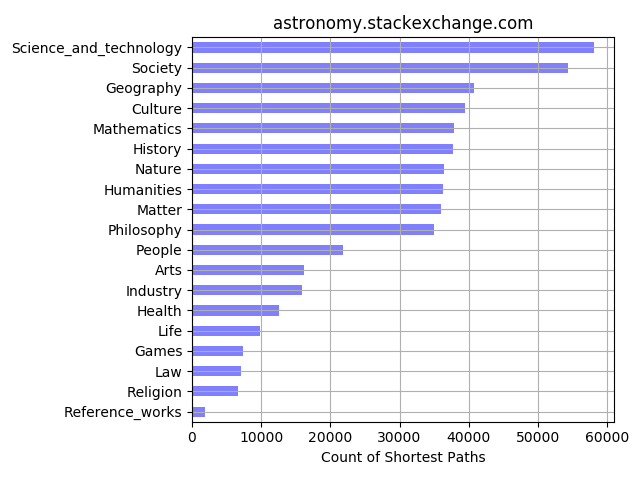
\includegraphics[width=1\linewidth]{imgs/path-counts/astronomy_stackexchange_com}
        \caption{Paths count for Astronomy}
        \label{fig:path-count-astronomy}
    \end{subfigure}%
    \begin{subfigure}{0.5\textwidth}
    \centering
        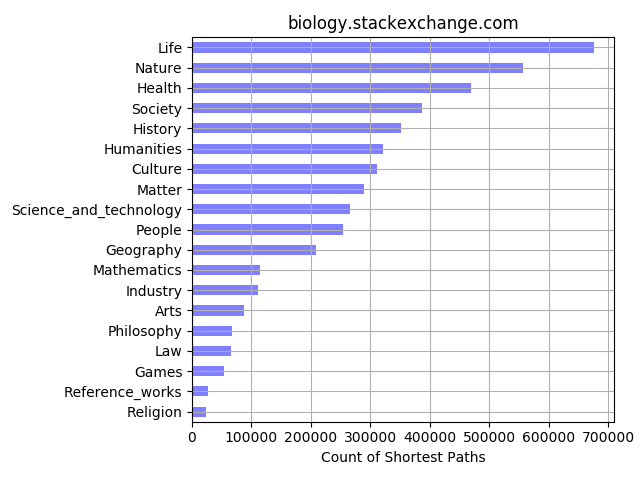
\includegraphics[width=1\linewidth]{imgs/path-counts/biology_stackexchange_com}
        \caption{Paths count for Biology}
        \label{fig:path-count-biology}
    \end{subfigure}
 
     \begin{subfigure}{0.5\textwidth}
    \centering
        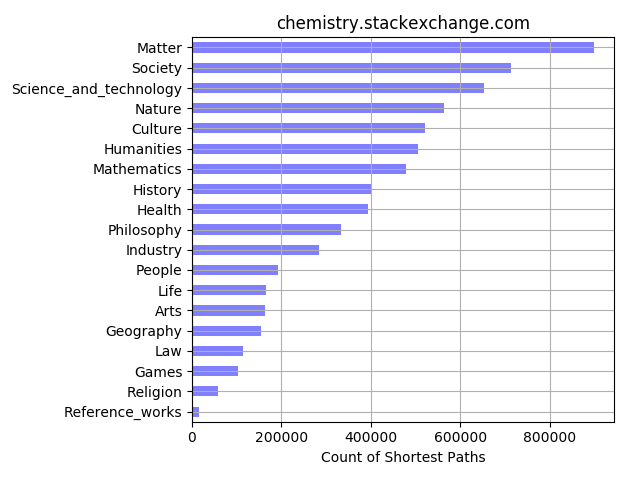
\includegraphics[width=1\linewidth]{imgs/path-counts/chemistry_stackexchange_com}
        \caption{Paths count for Chemistry}
        \label{fig:path-count-chemistry}
    \end{subfigure}%
    \begin{subfigure}{0.5\textwidth}
    \centering
        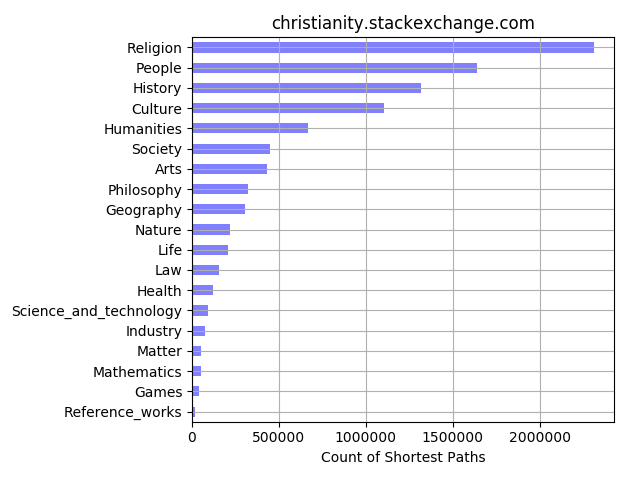
\includegraphics[width=1\linewidth]{imgs/path-counts/christianity_stackexchange_com}
        \caption{Paths count for Christianity}
        \label{fig:path-count-christianity}
    \end{subfigure}

        
     \begin{subfigure}{0.5\textwidth}
    \centering
        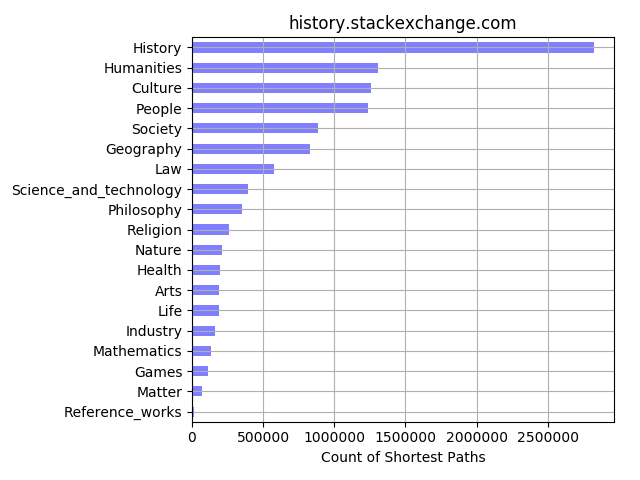
\includegraphics[width=1\linewidth]{imgs/path-counts/history_stackexchange_com}
        \caption{Paths count for History}
        \label{fig:path-count-history}
    \end{subfigure}%
    \begin{subfigure}{0.5\textwidth}
    \centering
        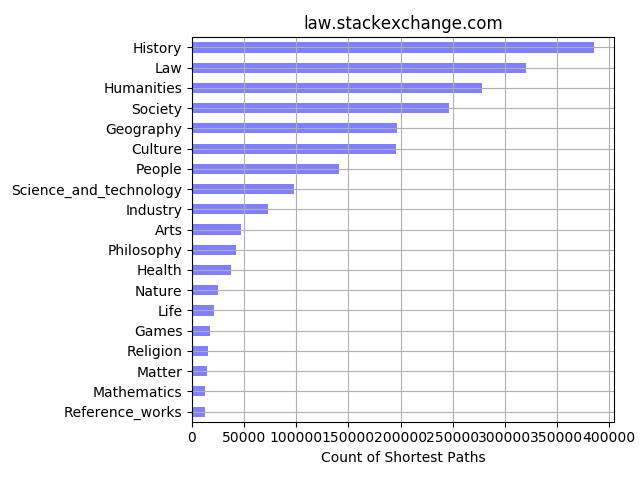
\includegraphics[width=1\linewidth]{imgs/path-counts/law_stackexchange_com}
        \caption{Paths count for Law}
        \label{fig:path-count-law}
    \end{subfigure} 

    \end{figure}
    
 \begin{figure}[H]
 \ContinuedFloat
    \centering
    \begin{subfigure}{0.5\textwidth}
    \centering
        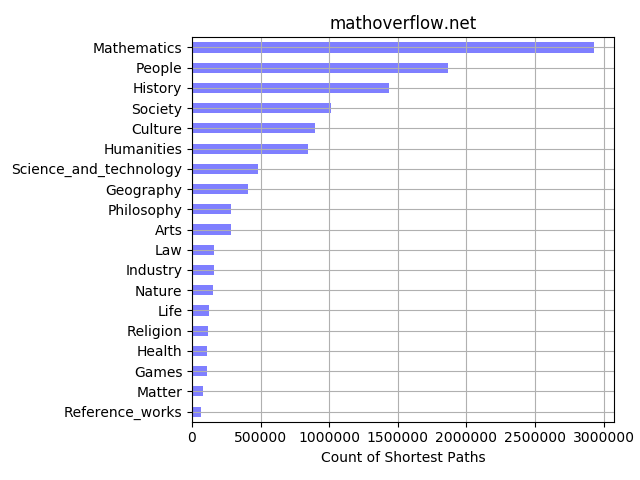
\includegraphics[width=1\linewidth]{imgs/path-counts/mathoverflow_net}
        \caption{Paths count for Math}
        \label{fig:path-count-math}
    \end{subfigure}%
    \begin{subfigure}{0.5\textwidth}
    \centering
        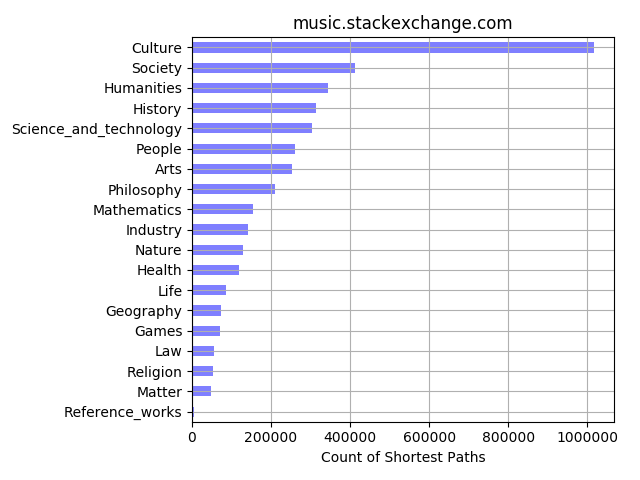
\includegraphics[width=1\linewidth]{imgs/path-counts/music_stackexchange_com}
        \caption{Paths count for Music}
        \label{fig:path-count-music}
    \end{subfigure}
 
     \begin{subfigure}{0.5\textwidth}
    \centering
        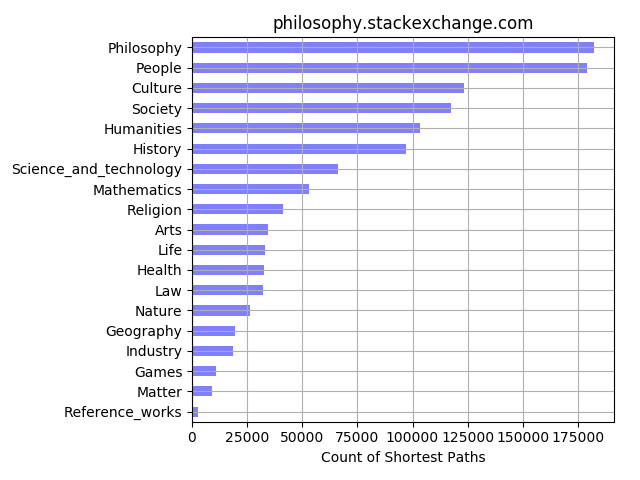
\includegraphics[width=1\linewidth]{imgs/path-counts/philosophy_stackexchange_com}
        \caption{Paths count for Philosophy}
        \label{fig:path-count-philosophy}
    \end{subfigure}%
    \begin{subfigure}{0.5\textwidth}
    \centering
        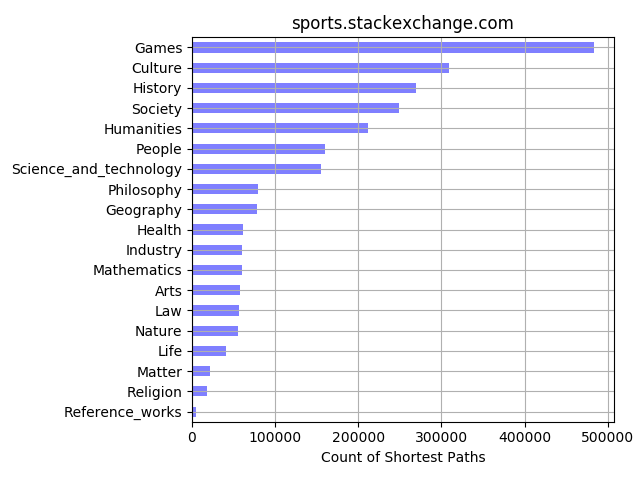
\includegraphics[width=1\linewidth]{imgs/path-counts/sports_stackexchange_com}
        \caption{Paths count for Sports}
        \label{fig:path-count-sports}
    \end{subfigure}
   
 
    \caption{The number of shortest paths through the proposed method. The X-axis shows the number of paths found for each top-level category (displayed on the Y-axis) }
    \label{fig:complete-path-count-distribution}
    
\end{figure}


The Culture category has several subcategories representing different aspects of Music as a form of expression (e.g., Music by Genre, Music by Culture, Music in Culture), and the technical aspects of Music as science (e.g., Musical Composition, Music Terminology).

Another particular case is the result for Law (\ref{fig:path-count-law}). As one of the 19 top-level is titled ``Law", it was expected that it would be the classification with the highest number of paths. It is however History, which appears with the highest degree, while Law appears second.

This can be explained as both concepts are closely related. New laws are passed in response to events occurring over the course of time - that is to say, history. One could argue that laws are a byproduct of history, but also that current laws will control future events (which, in turn, later become history themselves).

The example below of a genuine post (answer) extracted from the Law dataset illustrates how a topic related to Law is also connected to History. While there are the entities \textit{Treaties}, \textit{Court} and \textit{Domestic Law} that are strongly related to the concept of Law, there are also the terms \textit{Sovereign}, \textit{Maastricht Treaty} and \textit{Yugoslavia}, which are more strongly related to History. 

\begin{displayquote}
\say{One of the powers that sovereign nations have is to make treaties with other sovereign nations, these can be bi-lateral (as in the example you cite) or multi-lateral (like the Maastricht Treaty that binds the EU together). Once a treaty is agreed and signed it needs to ratified by each country which makes it part of the domestic law in that country: for your example, if India breaches the treaty it can be taken to court under the laws and in the courts of India or Pakistan(...). The worlds newest nation is, I believe, South Sudan, and one that has recently vanished is Yugoslavia. Laws are not contracts: contracts require consent of the parties, among other things., laws don't, they are imposed irrespective of consent.}
\end{displayquote}

As discussed in Chapter \ref{chapter:graph}, the \gls{wcg} presents the characteristics of a small-world network: a high level of connectivity between the nodes with relatively short paths.  To some extent, the whole knowledge encoded in Wikipedia is interconnected. As a result, although the frequency distribution of categories is more densely clustered close to the y-axis, and the distribution curve tapers along the x-axis,  it is important to note that there is at least a small percentage of relevance for each one of the 19 categories in the distribution for all ten datasets, as shown in figure \ref{fig:complete-path-count-distribution}. 

\section{\hspace*{3pt} Crowdsourcing study}

Due to the accessibility of established micro-task crowd-sourcing platforms such as Amazon’s Mechanical Turk\footnote{\url{www.mturk.com}} and CrowdFlower\footnote{\url{http://crowdflower.com}}, researchers are actively turning toward paid crowd-sourcing to solve data-centric tasks that require human input, such as building ground truths, validating results, and curating data \cite{7156008}.

\label{sec:crowd-sourcing-study}
In order to verify whether the classification generated by the applied method is coherent for real users, an experiment with human judges was conducted to ascertain the extent to which they agreed with the automatic classification result. To enable this comparison, Stack Exchange datasets were used in the experiment described in section \ref{section:proof-of-concept}.


\subsection{\hspace*{3pt} Experimental Design}

CrowdFlower was used to automatically allocate the available tasks to workers and to test them against known answers, namely the Gold Standard. Their performance on test questions indicates the extent to which the system trusts each worker -- if they become untrustworthy, the user is removed from the task, and their work is discarded.

For this experiment, topics defined as a Main topic classifications on Wikipedia (19 categories by the date of data extraction) were also considered as top-level categories. 

For each one of the ten communities, the experiment was run with 200 different random items extracted from the Stack Exchange dataset. Each worker was tasked with reading a randomly allocated text from the dataset, and ask to assert the extent to which they felt the text belonged to each one of the categories based on four options: i) not at all, ii) very little, iii) somewhat, or iv) to a great extent. 

As described in \cite{Gadiraju:2017}, prior research publications have referred to the importance of task clarity tangentially and stressed the positive impact of task design, clear instructions and descriptions on the quality of crowd-sourced work. For this reason, a detailed guide was provided for the workers, to ensure they would understand how to perform the task, with examples of good and bad judgments and also with a description of each one of the 19 categories. To make sure the task is perfectly designed, CrowdFlower platform offers a consulting service where the top-rated workers evaluate and give feedback on the quality of a given task. An example of the feedback given by this consulting service can be seen in figure \ref{fig:example-feedback}. The task description was adjusted according to the suggestions in the feedback by first providing more and contextualized examples, and second by explaining, for each test question, the reason why the alternatives were considered wrong or correct.  

To alleviate the intensive task of judging for 19 Categories, the participants were asked to evaluate the top-3 categories with the highest percentage distribution and two other random categories.  Figure \ref{fig:example-question} shows a real example of a task delivered to workers for the dataset Biology. The categories of Life, Health, and Nature are the top-3 categories with the highest degree of membership (see figure \ref{fig:path-count-biology}). The categories Religion and Games were randomly introduced into the survey. 

Random categories were included to validate whether, in addition to agreeing with the categories that appear with the highest distribution in the classification, the workers would also agree with those that do not belong to the most prominent categories. Moreover, this mechanism reinforces the verification of the validity of the judgments, since random categories cannot have a distribution of responses similar to those in the top-3 categories.

To select the participants able to perform the task (and to eliminate those with low performance), a series of 30 test questions for each stack exchange dataset were created. After executing the study with users in the crowd-sourcing platform, an analysis was performed in order to verify the extent to which these users agreed with the classification generated by the approach used with the ten datasets extracted from Q\&A communities.


\subsection{\hspace*{3pt} Quality Control}

When engaging a random collection of strangers to perform relevance evaluation, two primary concerns have risen:  i) How to ensure the workers performing the evaluation will have the necessary skill or knowledge? ii) How to ensure that the workers will make an high-quality effort to do the work, rather than clicking randomly on the responses?

To address these questions, parameters for ensuring quality regarding the workers and the experiment were defined:

\begin{enumerate}

\item Participation was restricted to workers from English-speaking countries to ensure that they understood the task and instructions adequately. 

\item Participation was restricted to Level-3 workers on CrowdFlower, meaning that only those who have completed over 100 test questions across hundreds of different types of tasks and have a near perfect overall accuracy were included. They are CrowdFlower's highest quality workers.

\item Each worker was restricted to a maximum of five judgments across all datasets, to minimize the number of workers trying to complete a disproportionately high number of tasks to maximize financial gain.

\item The value of 0.7 was asserted as the minimum level of agreement necessary for each row of evaluated text. In the case a row not reaching this value with the default number of three judgments, new judgments were requested until the level was reached. This value was chosen based on the suggestion of CrowdFlower platform. Values ranging from 0.71 to 0.80 were interpreted as substantial agreement \cite{mchugh2012interrater}.

Prior to running the experiment with all ten communities, the difference between the quality of judgments performed by elite workers and the judgments made by regular workers was evaluated. To perform this verification, the experiment was run using the Biology dataset with two different groups: one with regular workers exclusively, and the other with level-3 workers. Both were asked to judge the same set of 200 questions. 

\end{enumerate}

To compare the judgment made by the workers and the classification generated by the proposed method, the percentage of answers given in each of the categories of the scale (not at all, very little, somewhat and to a great extent) were aggregated for each of the evaluated texts. The precision, recall, and F-measure commonly used to verify the quality of \gls{ir} techniques, including text classifiers \cite{makhoul1999performance} were then calculated.

Precision measures the number of times a category was correctly predicted by the proposed method (True Positive) divided by the number of times that category was predicted in total (True Positive + False Positive). To maximize precision, the classifier must not fail to accurately classify the text entries in the dataset. Texts that should be assigned to one particular category according to the user study must be classified with the same category by the proposed automated approach. The main disadvantage of this metric is that it does not take into account the texts that should have been classified in a particular category, but were assigned to another one.

The recall bridges this gap by measuring the number of times a category has been assigned to a text by users (True Positive + False Negative), but the automatic classifier did not classify it correctly (False Negative). The disadvantage of this metric is that if the automated classifier did not classify any texts incorrectly, the recall would be maximum, even it was not efficient (because it also failed to sort correctly).

Measure F corresponds to the harmonic mean between precision and recall. With this information, the performance of the classifier can be asserted with an indicator only. The F-measure metric measures the efficiency of the classifier taking into account the error in both classes (True Positive and False Negative). It is necessary that the adjustment in both classes increase so that the metric increases. Considering that F-measure is an average, it gives a more accurate view of the efficiency of the classifier than just precision or recall.

\subsection{\hspace*{3pt} Results and Discussion}

1,265 unique workers participated in the final experiment, carried out between April and August 2018. The overall setup for the experiment is presented in table \ref{tab:experiment-overview}. A trusted judgment is an answer from a worker with an accuracy score higher than the minimum accuracy considered for this experiment (0.70), while an untrusted judgment is an answer from a worker whose accuracy score has fallen below this value.

\begin{table}[H]

\centering
\caption{Overall setup for the experiment with crowd workers}
\label{tab:experiment-overview}
\resizebox{\textwidth}{!}{%
\begin{tabular}{@{}llllll@{}}
\toprule
Community         & Trusted Judgments & Untrusted Judgments & Average Judgments per Row & Average Trust of Workers & Unique Workers \\ \midrule
Astronomy         & 640               & 36                  & 3.2000$\pm$0.73                      & 0.8651$\pm$0.061                               & 128            \\
Biology (Elite)   & 612               & 48                  & 3.0600$\pm$0.57                      & 0.8390$\pm$0.075                   & 122            \\
Biology (Regular) & 1040              & 278                 & 5.2000$\pm$1.78                      & 0.8366$\pm$0.073                   & 208            \\
Chemistry         & 751               & 12                  & 3.7550$\pm$1.22                      & 0.8197$\pm$0.087                     & 150            \\
Christianity      & 628               & 16                  & 3.1558$\pm$1.25                      & 0.8843$\pm$0.073                     & 125            \\
History           & 602               & 76                  & 3.0251$\pm$0.78                      & 0.7997$\pm$0.070                     & 120            \\
Law               & 601               & 0                   & 3.0050$\pm$0.66                      & 0.8831$\pm$0.094                     & 120            \\
Math              & 630               & 32                  & 3.1500$\pm$0.61                      & 0.9306$\pm$0.078                     & 126            \\
Music             & 602               & 28                  & 3.0100$\pm$1.10                      & 0.9137$\pm$0.092                     & 120            \\
Philosophy        & 717               & 108                 & 3.5850$\pm$0.83                      & 0.8376$\pm$0.068                     & 143            \\
Sports            & 629               & 32                  & 3.1608$\pm$0.12                      & 0.8349$\pm$0.073  & 125            \\ \bottomrule
\end{tabular}%
}
\end{table}

\subsubsection{\hspace*{3pt} Elite workers vs Regular workers}


A statistical test was applied to determine whether the results obtained in the answers given by the two groups can be considered significantly different from each other. The Wilcoxon-Mann-Whitney nonparametric statistical inference test was applied \cite{feltovich2003nonparametric} to compare the mean of two independent samples, as it does not require normality and homoscedasticity in the series of values compared. The level of significance was set at 95\%. The p-value evaluates the result of this statistical test. The lower the p-value, the higher the significance of the outcome. For a significance level of 95\%, if the p-value is smaller than 0.05, the responses observed for the two groups can be considered as distinct. 

A p-value of 0.267 ($\gg 0.05$) was obtained, meaning that there is no evidence of significant difference between the answers given by the two groups. Analyzing table \ref{tab:experiment-overview}, it is possible to see that regular users are less effective and thus more judgments are needed to achieve a reasonable level of agreement. Although the price paid to regular workers is lower by comparison to elite workers, a decision was made to admit only level-3 users.

\subsubsection{\hspace*{3pt} Human Judgment Analysis}

Figure \ref{fig:complete-crowd-distribution} shows the aggregated results of the participants' judgments for the categories in the Q\&A community datasets. The vertical axis presents the five categories involved in each study, three of which correspond to the categories with the highest degree of membership obtained in the experiment described in section \ref{section:proof-of-concept}. The other two are randomly inserted categories.

In the Astronomy (figure \ref{fig:percentage-distribution-astronomy}), Biology (figures \ref{fig:crowd-results-biology-1} and \ref{fig:crowd-results-biology-2}), Chemistry (figure \ref{fig:crowd-results-chemistry}), Christianity (figure \ref{fig:crowd-results-christianity}), Mathematics (figure \ref{fig:crowd-results-math}), Music (figure \ref{fig:crowd-results-music}) History (figure \ref{fig:crowd-results-history}), Philosophy (figure \ref{fig:crowd-results-philosophy}) and Sports (figure \ref{fig:crowd-results-sports}) communities, the category with the highest degree of relevance according to the proposed method were also the ones with the highest percentage of users asserting that they agreed with that category to a great extent. The most interesting findings regarding the comparison between the automatic classification and the answers given by users are highlighted below.

For the Law (figure \ref{fig:crowd-results-law}) category, while the proposed method identified History as the most relevant category in the dataset, the majority of users did not agree with this classification (97.70\% not at all). 
The users identified Law as the most relevant category in the dataset (55.31\% Somewhat and 42.95\% To a great extent), whereas the proposed method suggested it as the second most relevant category. 
From this observation, it is possible to infer that the automatic extraction of categories from the entities named in the text can capture more subtleties of the information, while the users tend to perceive (in most cases) only the knowledge explicitly described in the text.



 \begin{figure}[H]
    \centering
    \begin{subfigure}{0.5\textwidth}
    \centering
        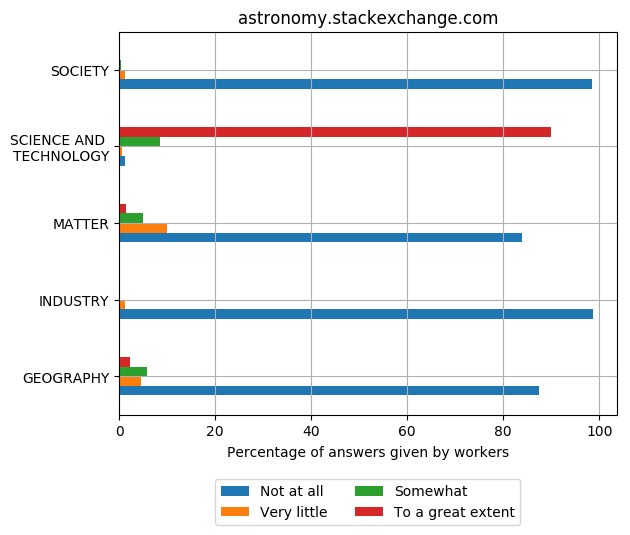
\includegraphics[width=1\linewidth]{imgs/crowd-results/astronomy_stackexchange_com}
        \caption{Distribution of Answers for Astronomy}
        \label{fig:crowd-results-astronomy}
    \end{subfigure}%
    \begin{subfigure}{0.5\textwidth}
    \centering
        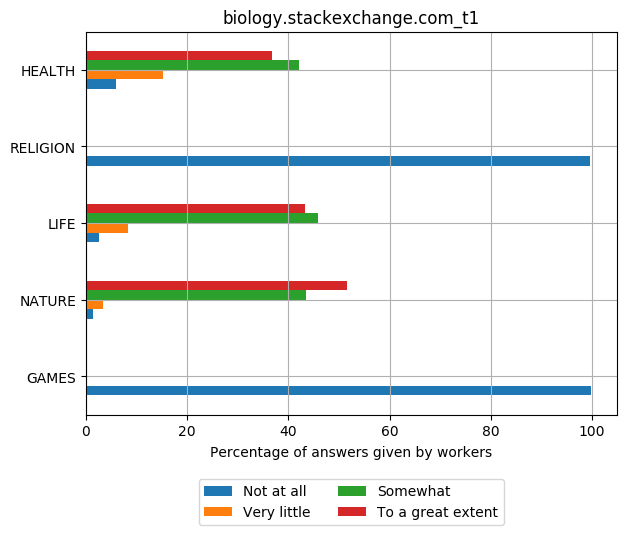
\includegraphics[width=1\linewidth]{imgs/crowd-results/biology_stackexchange_com_t1}
        \caption{Distribution of Answers for Biology (Regular)}
        \label{fig:crowd-results-biology-1}
    \end{subfigure}
 
     \begin{subfigure}{0.5\textwidth}
    \centering
        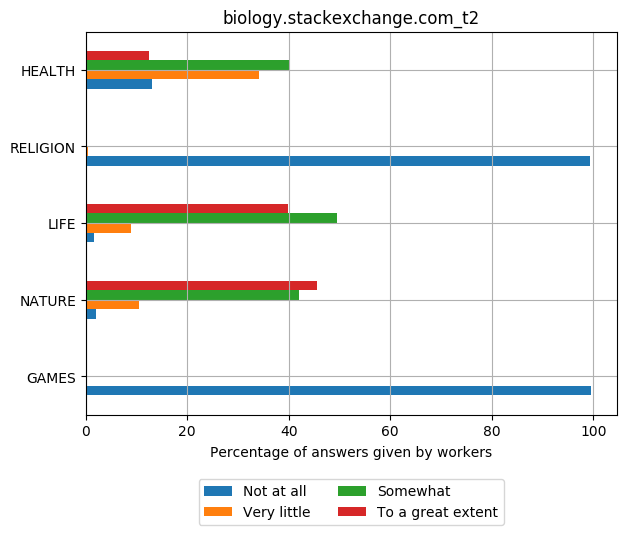
\includegraphics[width=1\linewidth]{imgs/crowd-results/biology_stackexchange_com_t2}
        \caption{Distribution of Answers for Biology (Elite)}
        \label{fig:crowd-results-biology-2}
    \end{subfigure}%
    \begin{subfigure}{0.5\textwidth}
    \centering
        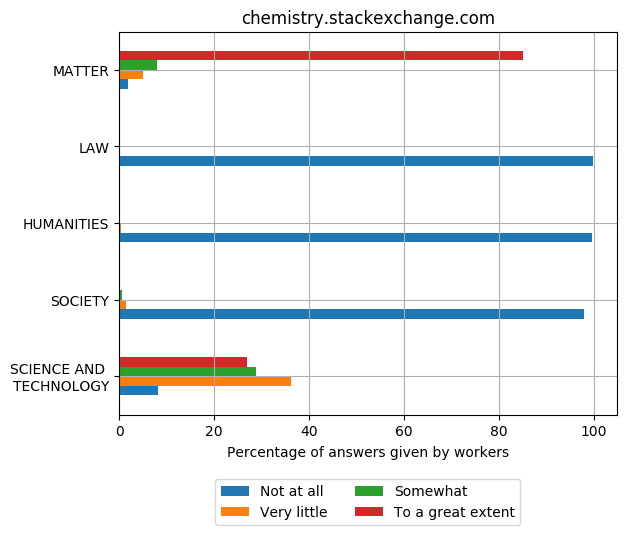
\includegraphics[width=1\linewidth]{imgs/crowd-results/chemistry_stackexchange_com}
        \caption{Distribution of Answers for Chemistry}
        \label{fig:crowd-results-chemistry}
    \end{subfigure}

        
     \begin{subfigure}{0.5\textwidth}
    \centering
        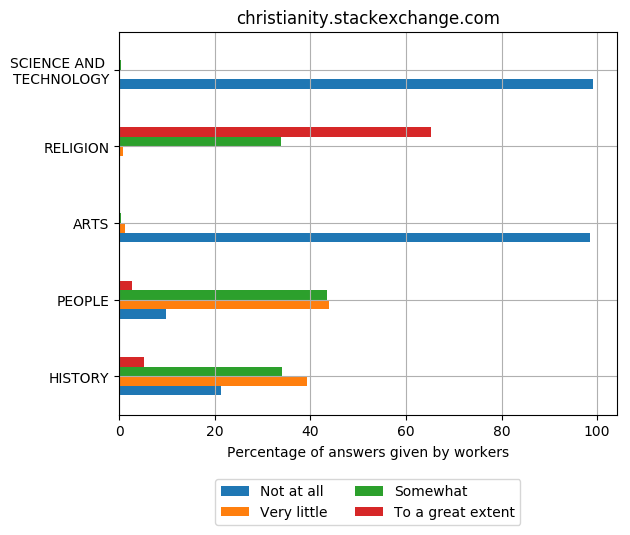
\includegraphics[width=1\linewidth]{imgs/crowd-results/christianity_stackexchange_com}
        \caption{Distribution of Answers for Christianity}
        \label{fig:crowd-results-christianity}
    \end{subfigure}%
    \begin{subfigure}{0.5\textwidth}
    \centering
        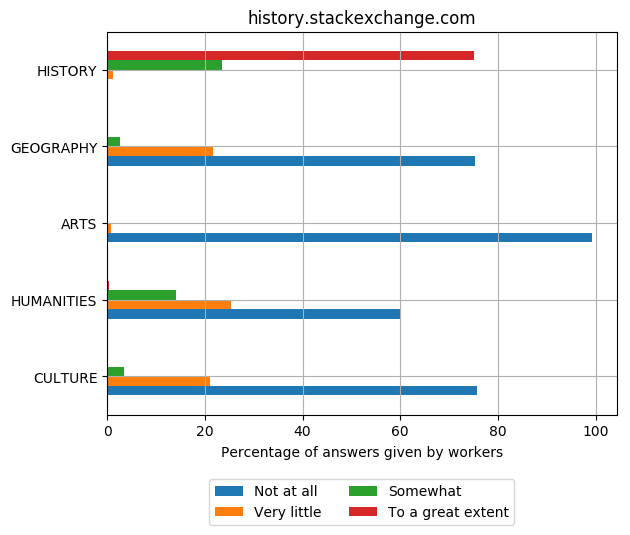
\includegraphics[width=1\linewidth]{imgs/crowd-results/history_stackexchange_com}
        \caption {Distribution of Answers for  History}
        \label{fig:crowd-results-history}
    \end{subfigure} 

    \end{figure}
    
 \begin{figure}[H]
 \ContinuedFloat
    \centering
    \begin{subfigure}{0.5\textwidth}
    \centering
        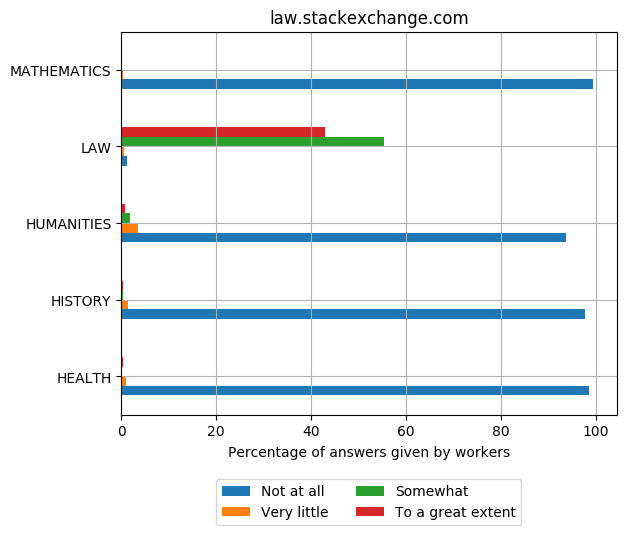
\includegraphics[width=1\linewidth]{imgs/crowd-results/law_stackexchange_com}
        \caption{Distribution of Answers for Law}
        \label{fig:crowd-results-law}
    \end{subfigure}%
    \begin{subfigure}{0.5\textwidth}
    \centering
        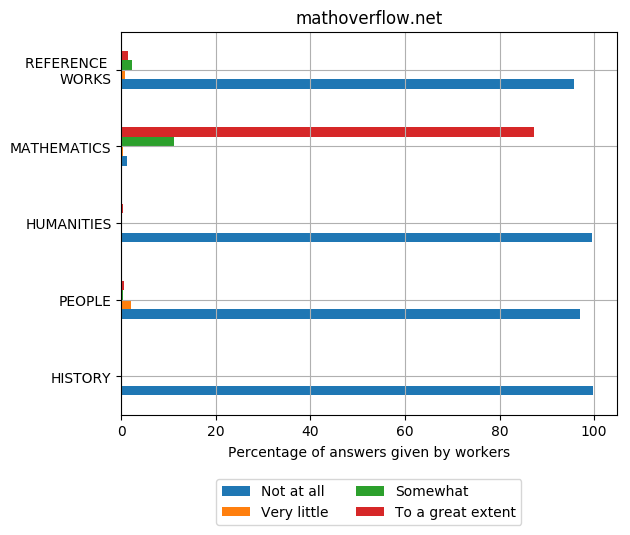
\includegraphics[width=1\linewidth]{imgs/crowd-results/mathoverflow_net}
        \caption{Distribution of Answers for Math}
        \label{fig:crowd-results-math}
    \end{subfigure}
 
     \begin{subfigure}{0.5\textwidth}
    \centering
        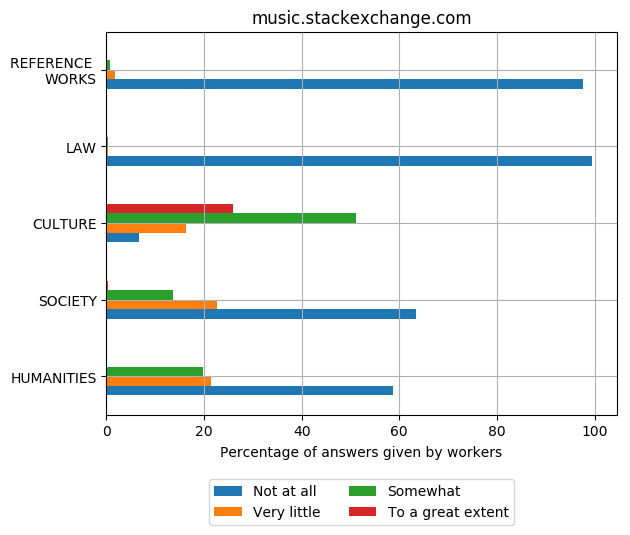
\includegraphics[width=1\linewidth]{imgs/crowd-results/music_stackexchange_com}
        \caption{Distribution of Answers for Music}
        \label{fig:crowd-results-music}
    \end{subfigure}%
    \begin{subfigure}{0.5\textwidth}
    \centering
        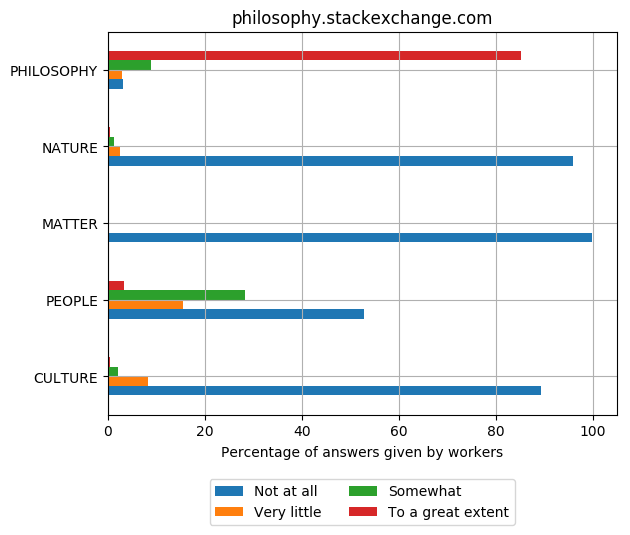
\includegraphics[width=1\linewidth]{imgs/crowd-results/philosophy_stackexchange_com}
        \caption{Distribution of Answers for Philosophy}
        \label{fig:crowd-results-philosophy}
    \end{subfigure}
    
     \begin{subfigure}{0.5\textwidth}
    \centering
        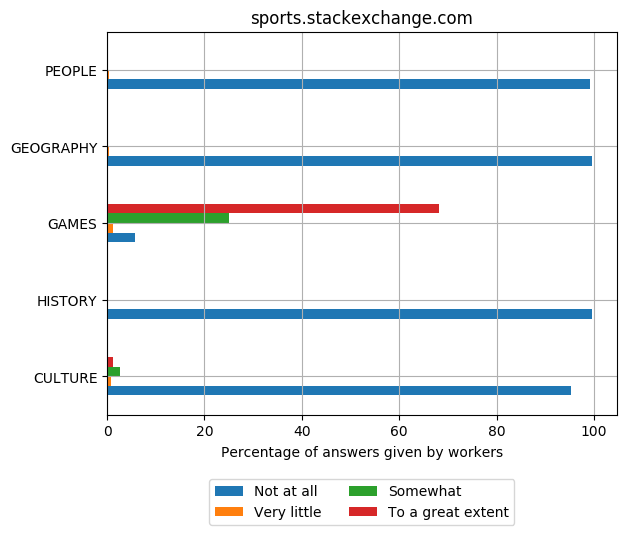
\includegraphics[width=1\linewidth]{imgs/crowd-results/sports_stackexchange_com}
        \caption{Distribution of Answers for Sports}
        \label{fig:crowd-results-sports}
    \end{subfigure}%
 \caption{Percentage distribution of answers given by crowd contributors for each one of the ten communities evaluated }
    \label{fig:complete-crowd-distribution}
    
\end{figure}
 
 \newpage
In the Astronomy (figure \ref{fig:crowd-results-astronomy}) community, the three most relevant categories were Science and Technology, Society, and Geography respectively. The categories inserted randomly were Industry and Matter. For the most relevant category (Science and Technology), the vast majority of users agreed with the classification generated by the proposed method (89.86\% To a great extent, 8.52\% Somewhat, and 4.57\% Very little).

The category Society was the second most relevant according to the automatic classification, but it was not identified by the users (87.51\% Not at all). This can be explained by the fact that users identify categories superficially, based on their prior knowledge, but fail to recognize more tacit subjects that permeate the discussions. A good example that justifies the presence of the Society category in the automatic classification is the presence of several inquiries regarding the Geocentric Model, that is linked to the categories History of astrology, History of astronomy and Obsolete scientific theories, and indirectly connected to the category Society.
However, users tend to answer that there is no relationship at all to the category Society in these discussions.

Although the category Matter was not one of the top 3 most relevant according to the proposed method's classification, it was identified as such by some users (9.88\% Very little, 4.94\% Somewhat and 1.35\% To a great extent). The many discussions in the Astronomy community regarding the existence of carbon, water and other elements in the surface and the atmosphere of planets are the likely explanation for this phenomenon. 

In the History community dataset (figure \ref{fig:crowd-results-history}), although the proposed method did not identify the category Geography as one of the top-3 most relevant categories (hence, it was randomly inserted in the experiment for this dataset), a considerable number of users asserted some degree of relevance to this category (21.70\% Very little,  2.68\% Somewhat and 0.24\% To a great extent). 

To extend the analysis, the precision, recall and F-measure were calculated for each of the texts judged by the workers and the automatic classification. Table \ref{tab:row-wise-comparison} shows the summarized results. For this analysis, two levels of comparison were considered - they are identifiable in table \ref{tab:row-wise-comparison} as L1 and L2. The first level (L1) considered the proposed method to be correct when for a given text the category with the highest level of relevance was also identified by the user as related to the text to a great extent. The second level of comparison (L2) considered the proposed classification as correct when the user identified the text as related somewhat or to a great extent with the category suggested as the most relevant by the proposed method. 



\begin{table}[H]
\centering
\caption{Values of precision, recall and F-measure when comparing our classification and the judgments made by workers in the crowdsourcing study}
\label{tab:row-wise-comparison}
\resizebox{\textwidth}{!}{%
\begin{tabular}{@{}lllllll@{}}
\toprule
& \multicolumn{3}{c}{L1} & \multicolumn{3}{c}{L2} \\ \midrule
Community                          & Precision    & Recall   & F-Measure   & Precision    & Recall    & F-Measure    \\
astronomy.stackexchange.com        & 0.9423       & 0.2022   & 0.3330      & 0.9872       & 0.1935    & 0.3235       \\
biology.stackexchange.com          & 0.4170       & 0.3311   & 0.3691      & 0.9064       & 0.3492    & 0.5041       \\
chemistry.stackexchange.com.csv    & 0.8571       & 0.3111   & 0.4565      & 0.9524       & 0.3160    & 0.4746       \\
christianity.stackexchange.com.csv & 0.6815       & 0.5951   & 0.6353      & 0.9960       & 0.5731    & 0.7275       \\
history.stackexchange.com.csv      & 0.7528       & 0.6526   & 0.6991      & 0.9925       & 0.6559    & 0.7899       \\
law.stackexchange.com.csv          & 0.0149       & 0.6667   & 0.0292      & 0.0299       & 0.6667    & 0.0571       \\
mathoverflow.net.csv               & 0.8896       & 0.6361   & 0.7418      & 0.9955       & 0.6314    & 0.7727       \\
music.stackexchange.com.csv        & 0.2760       & 0.8019   & 0.4106      & 0.8019       & 0.7816    & 0.7917       \\
philosophy.stackexchange.com.csv   & 0.9081       & 0.3889   & 0.5446      & 0.9622       & 0.3732    & 0.5378       \\
sports.stackexchange.com.csv       & 0.7372       & 0.5479   & 0.6286      & 0.9805       & 0.5331    & 0.6907       \\ \bottomrule
\end{tabular}%
}
\end{table}
For the majority of datasets,  high precision ($>0.70$) and a moderate recall ($>0.50$) were obtained, meaning that the proposed method identifies one category as the most relevant when the users pointed it as related to a great extent with the text. The users did however sometimes identify a category that was not the most relevant according to the proposed method as the one with highest relation to the text.

In the Biology and Music datasets, when considering L1 as the basis for the comparison, a low value for precision was obtained. This is mainly because there is a better distribution of answers as ``to a great extent" along the 3 most relevant categories pointed out by the proposed method than in the other datasets (figures \ref{fig:crowd-results-biology-2}, \ref{fig:crowd-results-biology-2} and \ref{fig:crowd-results-music}). If we consider L2 as the basis of the comparison instead, the precision increases significantly for both datasets. 

The Law dataset is the only one to show low values for precision for both L1 and L2. This is because while the proposed method identified the category History as the most relevant, the majority of users identified only the category Law as being related to the texts to a great extent.

%\section{\hspace*{3pt} Experiment with the 20 NewsGroup Dataset}

%Os experimentos descritos nas seções \ref{sec:}

%Finally, we have used the document representation proposed by our approach in the classification of documents of a classic dataset employing a probabilistic classification algorithm, with the intent to compare and discuss the results regarding a related work.

%\subsection{\hspace*{3pt} 20 NewsGroups}

%The 20 Newsgroups dataset is a collection with approximately 20,000 documents from the Usenet discussion forum. The documents in this collection are divided into 20 categories related to the following subjects: computers, business, religion, politics, science, and fun. The distribution of documents among categories is regular, i.e., categories have approximately the same number of documents, and each document belongs to only one category.







%\begin{figure}[H]
%\centering
%  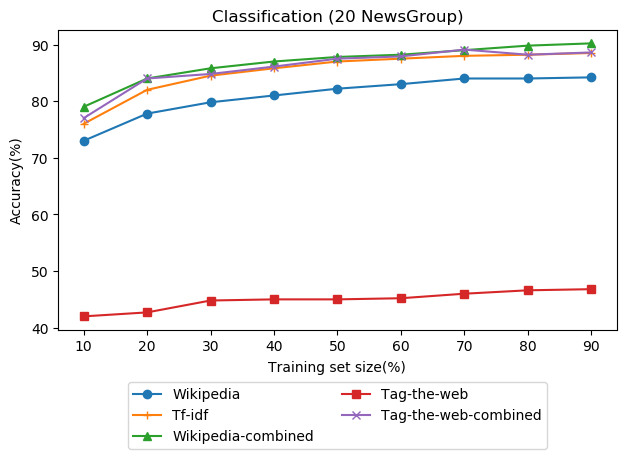
\includegraphics[width=\linewidth]{comparison.png}
%  \caption{Classification accuracy in 20 Newsgroups at various training set sizes compared %to \cite{schonhofen2009identifying} }
%  \label{fig:example-comparison}
%\end{figure}


%A common criticism of naïve Bayesian text classifiers is that they make the naïve assumption that words are independent of each other

